\documentclass[journal]{IEEEtran}

\usepackage{graphicx}
\usepackage{graphicx}
\graphicspath{{img/}}
\DeclareGraphicsExtensions{.pdf,.jpeg,.png}

% correct bad hyphenation here
\hyphenation{op-tical net-works semi-conduc-tor}

\usepackage[style= ieee, 
            urldate=comp,
            backend= biber]{biblatex}
\usepackage{xpatch}
\usepackage{url}
\usepackage{siunitx}

\begin{filecontents*}{\jobname.bib}
@misc{SPOF,
 title={Definition Single Point of Failure},
 url={https://en.wikipedia.org/wiki/Single_point_of_failure},
 note={(Date last accessed 11-August-2017)},
 }
 
@BOOK{Rastocny2013,
  author = {Rástočný, Karol and Ždánsky, Juraj},
  title = {Riadiace systémy so safety PLC},
  year = {2013},
  pages = {203},
  publisher = {VÚŽ Praha},
  owner = {Jaroslav Fait},
  timestamp = {2017.05.03},
  url = {http://librarian/stable.php?id=261}
}

\end{filecontents*}
\addbibresource{\jobname.bib}

\begin{document}
%
% paper title
\title{Design Power Supply with Uvervoltage Protection \\
       Acceptable for SIL4  application According EN50129}

\author{Jaroslav~Fait} 

% The paper headers
\markboth{WayGuard Project: RA\_HW002,~Vol.~1, No.~1, August~2017}%
{Shell \MakeLowercase{\textit{et al.}}: Bare Demo of IEEEtran.cls for IEEE Journals}

% make the title area
\maketitle

% As a general rule, do not put math, special symbols or citations
% in the abstract or keywords.
\begin{abstract}
  During fault conditions, most power supplies have the potential to deliver higher output
  voltages than those normally specified or required. In unprotected equipment, it is possible
  for output voltages to be high enough to cause internal or external equipment damage. To
  protect the equipment under these abnormal conditions, it is common practice to provide
  some means of overvoltage protection within the power supply.
\end{abstract}

% Note that keywords are not normally used for peerreview papers.
\begin{IEEEkeywords}
  SIL4, WayGuard, Bistabil relay
\end{IEEEkeywords}




% For peer review papers, you can put extra information on the cover
% page as needed:
% \ifCLASSOPTIONpeerreview
% \begin{center} \bfseries EDICS Category: 3-BBND \end{center}
% \fi
%
% For peerreview papers, this IEEEtran command inserts a page break and
% creates the second title. It will be ignored for other modes.
\IEEEpeerreviewmaketitle


\section{Single Points of Failure in a simple setup}
  Systems can be made robust by adding redundancy in all potential SPOFs (single point of failure) 
  \cite{SPOF}. For example on the figure \ref{HW002:fig006}, two sensors are powered by simplex 
  element - power source. If the power supply breaks (overvoltage/undervoltage), it can compromise 
  any safety margin gained in using dual sensors. 
  
  \begin{figure}[!ht] %\ref{HW002:fig006}
    \centering
    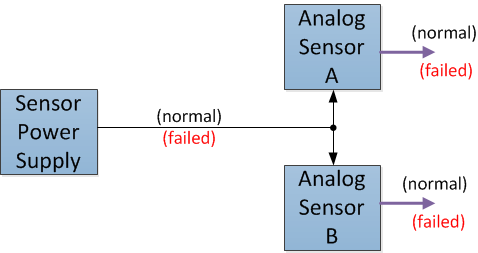
\includegraphics[width=0.8\linewidth]{fig_HW006.png}
    \caption{Simplex component failure may brings in matching but incorrect results in the dual 
             sensors}
    \label{HW002:fig006}
  \end{figure}
  
    Redundancy can be achieved at various levels. The assessment of a potential SPOF involves 
    identifying the critical components of a complex system that would provoke a total systems 
    failure in case of malfunction. Highly reliable systems should not rely on any such individual 
    component.

\section{Dual Computer Architecture}
  
  When microcomputers were introduced in mid 1980s, diagnostic functions became the main force of 
  the CPUs. In applying microcomputers to railway signalling, conventional safety measures based on 
  the asymmetric nature of component failure modes are not available. Instead, however, 
  microcomputers enable high-frequency diagnosis, and this leads to composite fail-safety and 
  reactive fail-safety as well. 
  
  The Dual Computer Architecture is the adoption of identical duplicate CPU configuration 
  (identical software).  Computer hardware, power supply, and interconnects (and
  sensors) are all duplicated, as is shown in figure \ref{HW002:fig005}. Each of the groups is 
  referred to as a channel.
  

  \begin{figure}[!ht] %\ref{HW002:fig005}
    \centering
    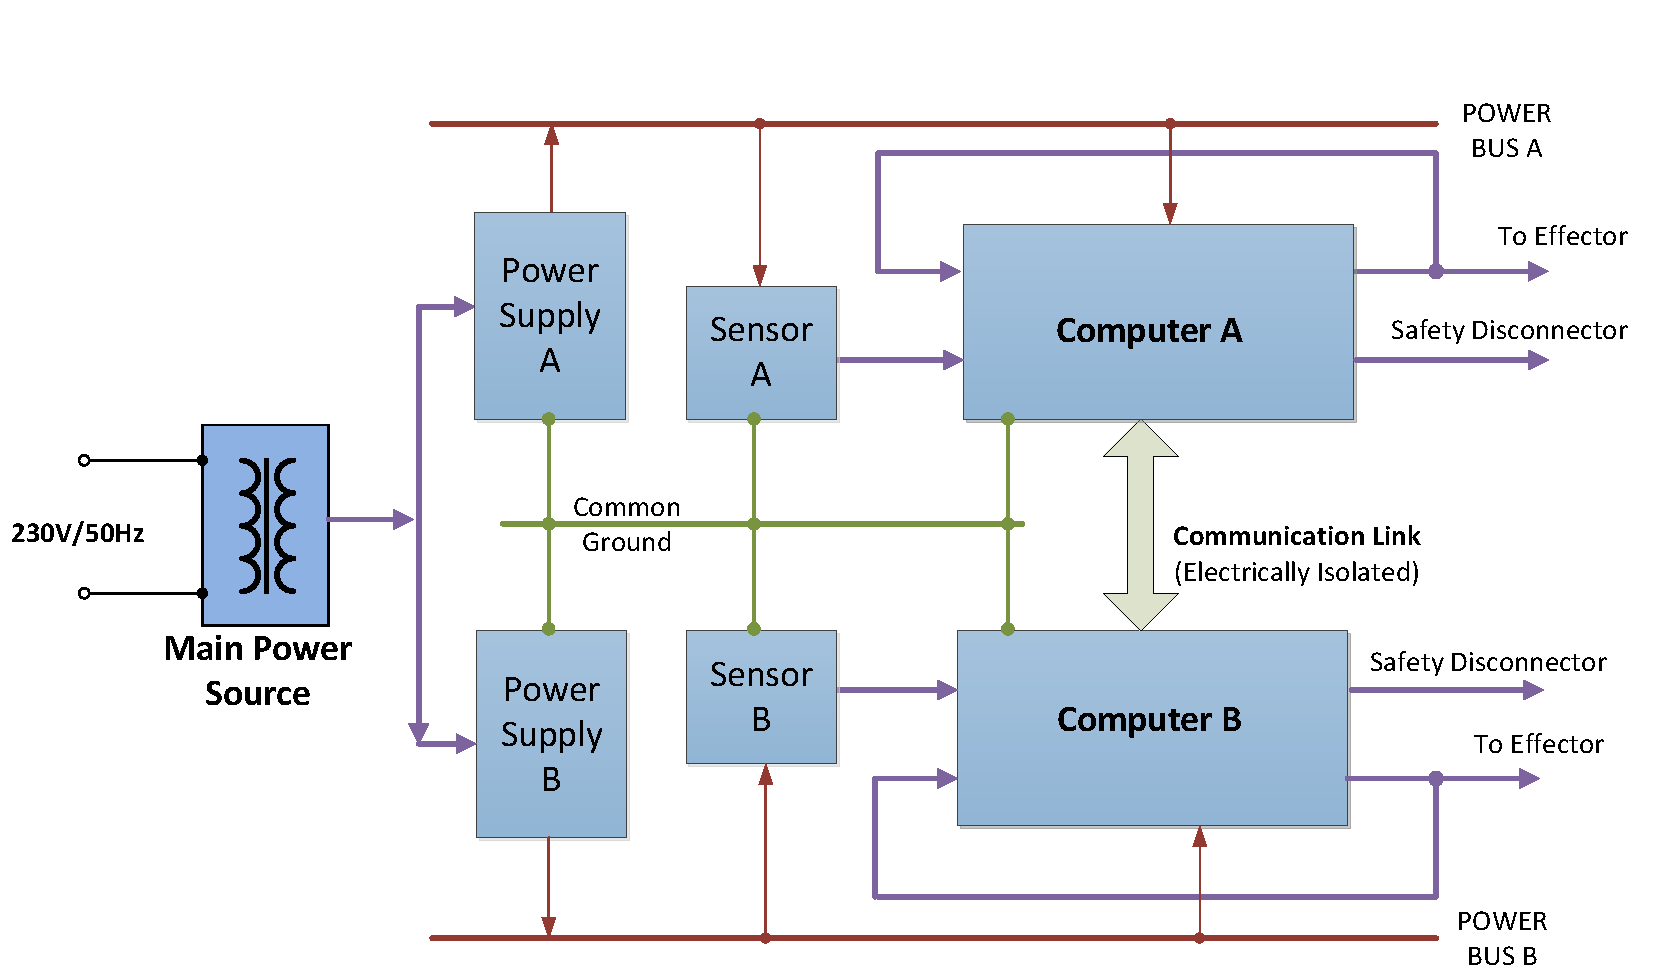
\includegraphics[width=1\linewidth]{fig_HW005.pdf}
    \caption{Redundant CPU Architecture }
    \label{HW002:fig005}
  \end{figure}

  Assumption:
  \begin{enumerate}[noitemsep]
    \item Hardware in the channels is independent: A hardware failure in a channel has no effect 
          on the correct performance of other channels.
    \item The communication path is electrically isolated from the computers: A hardware failure 
          (such as a short circuit) in the connecting path will not propagate to computers.
   \end{enumerate}
   
  In safety discussion, whether or not a safe state can be defined also plays a big role power 
  supply concept, because wrong supplying can easy lead to \emph{common cause failure}.
  
  A common cause failure occurs when several failures have the same origin. Common cause failures 
  are either common event failures, where the cause is a single external event, or common mode 
  failures, where two systems fail in the same way for the same reason. Common mode failures can 
  occur at different times because of a design defect or a repeated external event
  
  For example overvoltage on the Main Power Supply's output on figure \ref{HW002:fig005} can leads 
  to same failure of all Auxiliary Power supplies, which can compromise all parts of the Fail-Safe. 
  
  The benefit of component duplication can be defeated by \emph{common-cause failure} (CCF) or 
  \emph{common-mode failures} (CMF)

\section{Types of overvoltage protection}
  Overvoltage protection techniques fall broadly into three categories:
  \begin{itemize}
   \item Type 1: simple SCR “crowbar” overvoltage protection
   \item Type 2: overvoltage protection by voltage clamping techniques
   \item Type 3: overvoltage protection by voltage limiting techniques
  \end{itemize}

  The technique chosen will depend on the power supply topology, required performance, and cost.
  
  \subsection{Type 1, SCR “Crowbar” overvoltage protection}
    \emph{Crowbar protection} is a fail-safe protection mechanism which pulls the voltage below 
    the trigger level, usually close to ground. A clamp prevents the voltage from exceeding a 
    preset level. Thus, a crowbar will not automatically return to normal operation when the 
    overvoltage condition is removed; power must be removed entirely to stop its conduction. 
    Crowbar protection can also refer to a circuit which has its sole purpose to cause a fuse to 
    blow by subjecting it to high current.
  
    \begin{figure}[!ht] %\ref{HW002:fig003}
      \centering
      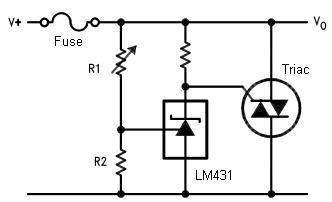
\includegraphics[width=0.6\linewidth]{fig_HW003.jpg}
      \caption{Simple crowbar protection with triac}
      \label{HW002:fig003}
    \end{figure}
    
    An example crowbar circuit is shown in the figure \ref{HW002:fig003}. This particular circuit 
    uses an \texttt{LM431} adjustable zener regulator to control the gate of the \texttt{TRIAC}. 
    The resistor divider  of \texttt{R1} and \texttt{R2} provide the reference voltage for the 
    \texttt{LM431}. The divider is set so that during normal operating conditions, the voltage 
    across  \texttt{R2} is slightly lower than \(V_{ref}\) of the \texttt{LM431}. Since this 
    voltage is below the minimum reference voltage of the \texttt{LM431}, it remains off and very 
    little current is conducted through the zener and cathode resistor. If the cathode resistor is 
    sized accordingly, very little voltage will be dropped across it and the \texttt{TRIAC} gate 
    terminal will be essentially at the same potential as MT1 (main terminal 1), keeping the 
    \texttt{TRIAC} off. If the supply voltage increases, the voltage across \texttt{R2} will exceed 
    \(V_{ref}\) and the zener will begin to regulate voltage, drawing more current through it. The 
    voltage at the gate terminal will be pulled down to \(V_Z\) (the zener voltage), exceeding the 
    gate trigger voltage of the \texttt{TRIAC}and latching it on.
    
    Similar function can be seen on figure \ref{HW002:fig004}, where is used thyristor. 
    
    \begin{figure}[!ht] %\ref{HW002:fig004}
      \centering
      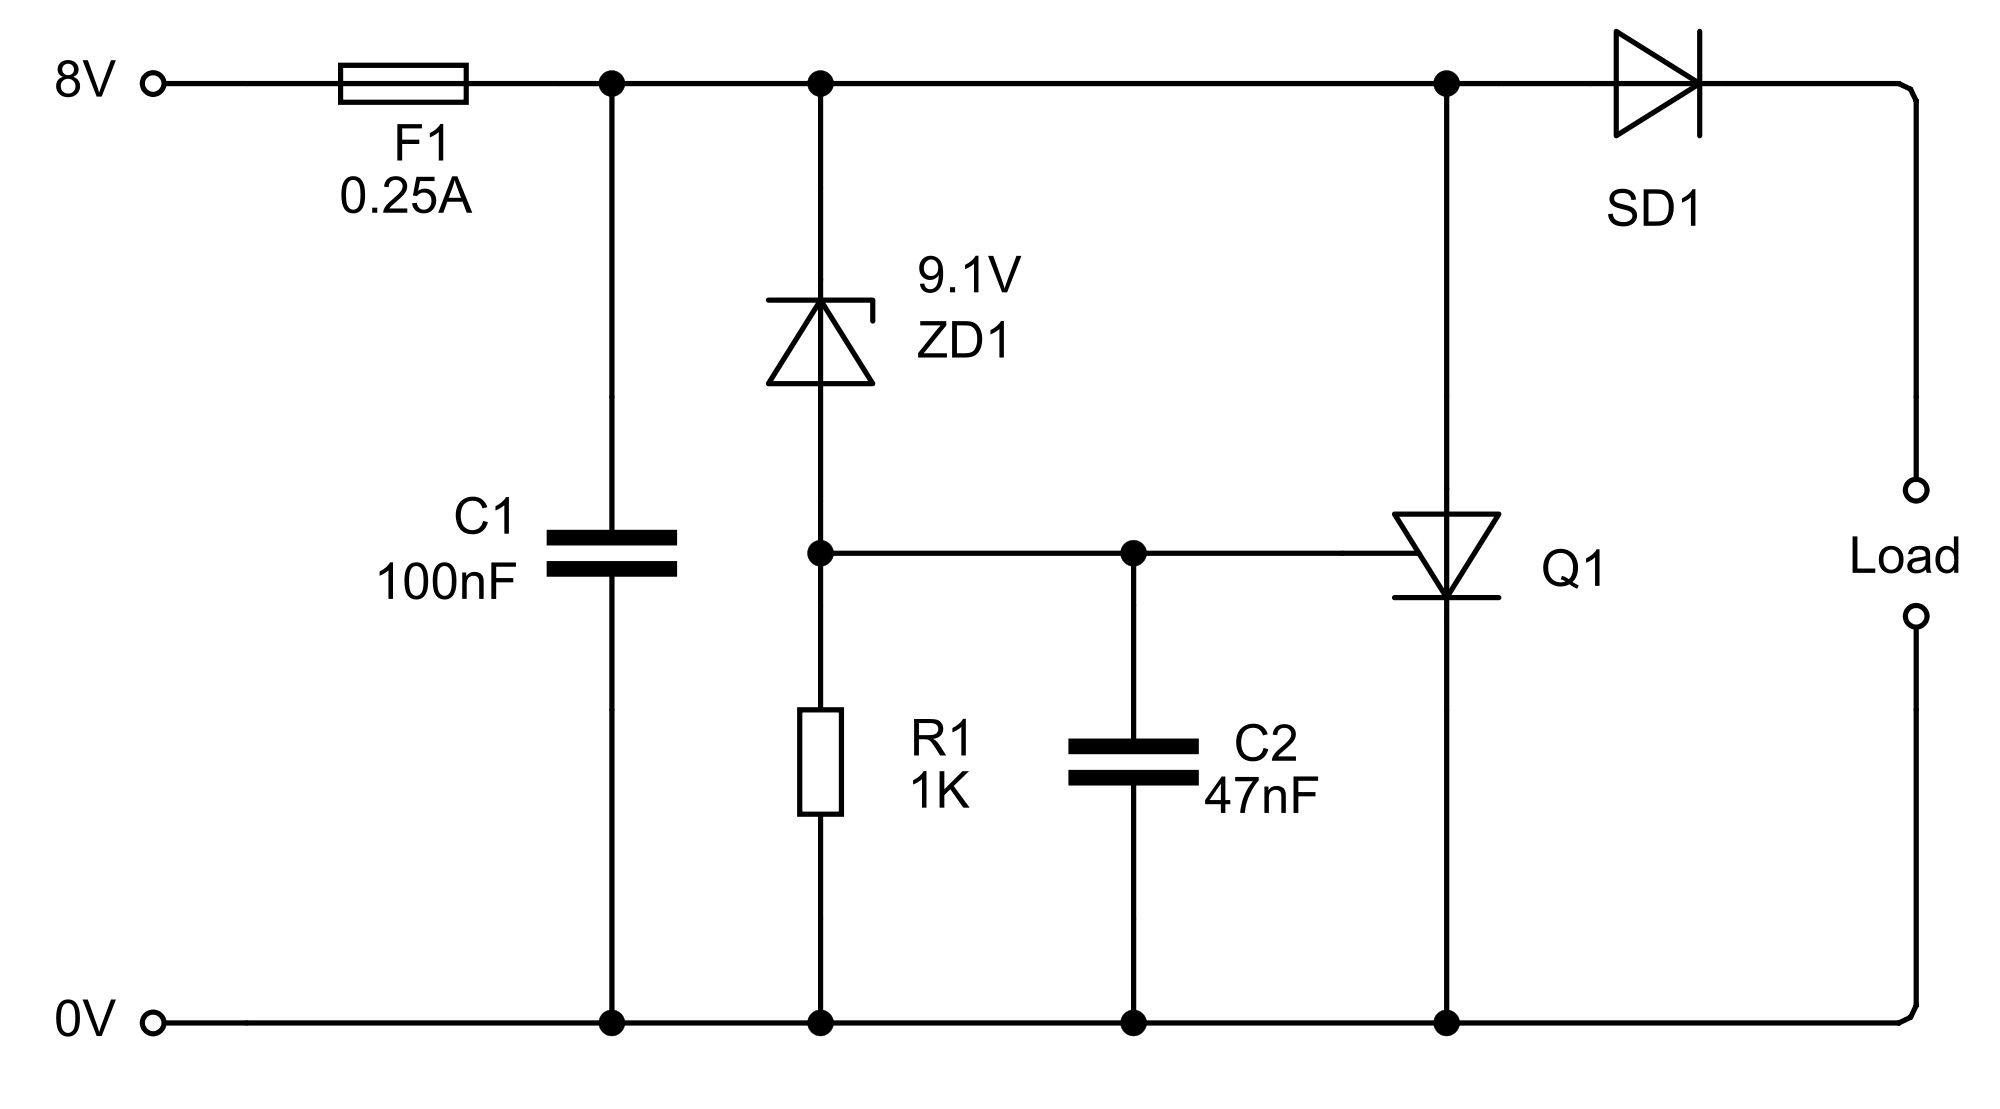
\includegraphics[width=0.6\linewidth]{fig_HW004.png}
      \caption{Simple Crowbar Protection with thyristor}
      \label{HW002:fig004}
    \end{figure}
    
    Crowbar circuits are so named because their activation is similar in effect to dropping a 
    crowbar across bus bars (heavy duty power supply lines).

    \subsection{Linear regulator with "crowbar" protection}

    Let's look at the concrete implementation of the linear power supply equipped with 
    shortcircuiting device (SCR), which is activated when the overvoltage stress exceeds a preset 
    limit for a defined time period. When the SCR is activated, it short-circuits the output of the 
    power supply to the common return line, thus collapsing the output voltage. A typical simple 
    SCR “crowbar” overvoltage protection circuit connected to the output of a linear regulator is 
    shown in Fig \ref{HW002:fig007}
    
    \begin{figure}[!ht] %\ref{HW002:fig007}
      \centering
      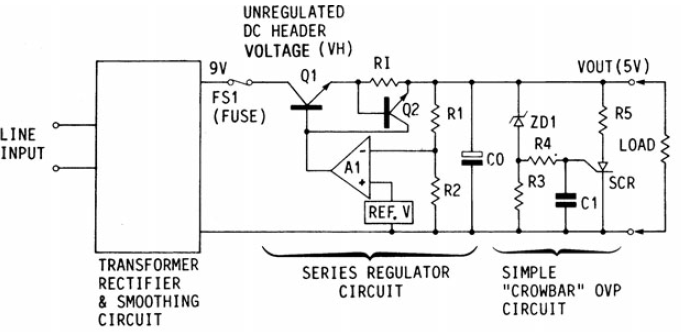
\includegraphics[width=1\linewidth]{fig_HW007.png}
      \caption{Simple Crowbar Protection with thyristor}
      \label{HW002:fig007}
    \end{figure}
    
    The most catastrophic failure condition would be a short circuit of the series regulating
    device Q1, so that the higher unregulated header voltage VH is now presented to the output
    terminals. Under such fault conditions, both voltage control and current limit actions are
    lost, and the “crowbar” SCR must be activated to short-circuit the output terminals.
    In response to an overvoltage fault, the “crowbar” circuit responds as follows: As the
    voltage across the output terminals rises above the “crowbar” actuation voltage, zener
    diode ZD1 conducts driving current via R4 into the SCR gate delay capacitor C1. After a
    short delay period defined by the values of C1, R4 and the applied voltage, C1 will have
    charged to the gate firing voltage (0.6 V), and the SCR will conduct to short-circuit the
    output terminals via the low-value limiting resistor R5. However, a large current now flows
    from the unregulated DC input through the shunt-connected “crowbar” SCR. To prevent
    over-dissipation in the SCR, it is normal, in linear regulators, to fit a fuse FS1 or circuit
    breaker in the unregulated DC supply. If the series regulator device Q1 has failed, the fuse
    or circuit breaker now clears, to disconnect the prime source from the output before the
    “crowbar” SCR is destroyed.

    \begin{figure}[!ht] %\ref{HW002:fig008}
      \centering
      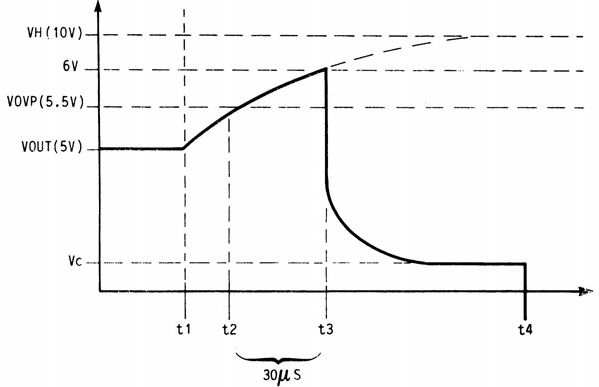
\includegraphics[width=1\linewidth]{fig_HW008.png}
      \caption{Typical performance characteristic of a delayed “crowbar” circuit.}
      \label{HW002:fig008}
    \end{figure}
    
    The design conditions for such a system are well defined. It is simply necessary to select
    an SCR “crowbar” or other shunt device that is guaranteed to survive the fuse or circuit
    breaker’s “let-through” energy. With SCRs and fuses, this “let-through” energy is normally
    defined in terms of the I 2t product, where I is the fault current and \(t\) the fuse or breaker
    clearance time.
    
    Crowbar protection is often preferred and hence specified by the systems engineer
    because it is assumed to provide full protection (even for externally caused overvoltage
    conditions). However, full protection may not always be provided, and the systems engineer
    should be aware of possible anomalous conditions.
    
    In standard, “off-the-shelf” power supply designs, the crowbar SCR is chosen to protect
    the load from internal power supply faults. In most such cases, the maximum let-through
    energy under fault conditions has been defined by a suitably selected internal fuse. The
    power supply and load are thus \SI{100}{\percent} protected for internal fault conditions. 
    However, in a complete power supply system, there may be external sources of power, which may
    become connected to the terminals of the SCR-protected power supply as a result of some
    system fault. Clearly, the fault current under these conditions can exceed the rating of the
    “crowbar” protection device, and the device may fail (open circuit), allowing the overvoltage
    condition to be presented to the load.
    
    Such external fault loading conditions cannot be anticipated by the power supply
    designer, and it is the responsibility of the systems engineer (user) to specify the worst-case
    fault condition so that suitable “crowbar” protection devices can be provided.
    
  \nocite{*}
\printbibliography
\end{document}